% !TEX root = main.tex

%%%%%%%%%%%%%%%%%%%%%%%%%%%%%%%%%%%%%%%%%%%%%%%%%%%%%%%%%%%%%%%%%%%%%%%%%%%%%%%%%%%%%%%%%%%%%%%%
\section{結果}
%%%%%%%%%%%%%%%%%%%%%%%%%%%%%%%%%%%%%%%%%%%%%%%%%%%%%%%%%%%%%%%%%%%%%%%%%%%%%%%%%%%%%%%%%%%%%%%%

\subsection{予測波形}
シミュレーションを行った回路を図5,図6に示す.
\begin{figure}[H]
    \begin{center}
        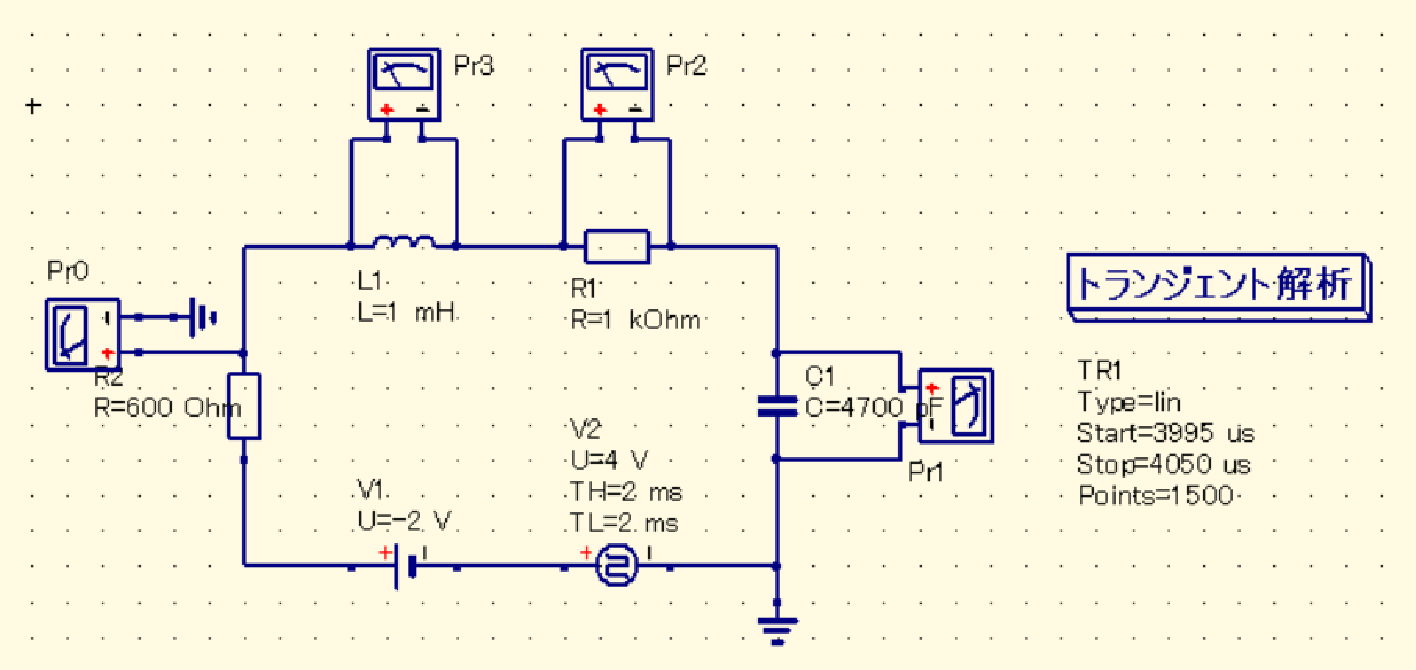
\includegraphics[keepaspectratio, scale=0.7]{circuit1.pdf}
        \caption{測定回路1}
    \end{center}
\end{figure}

\begin{figure}[H]
    \begin{center}
        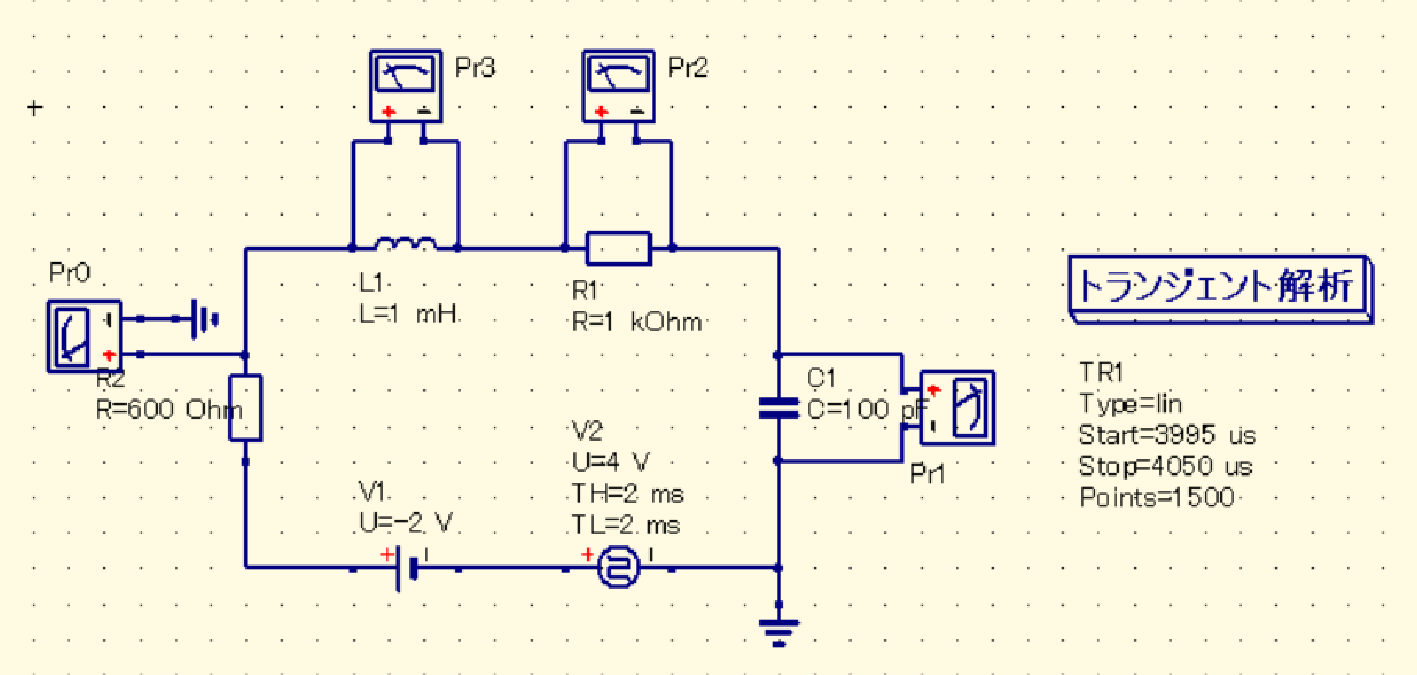
\includegraphics[keepaspectratio, scale=0.7]{circuit2.pdf}
        \caption{測定回路2}
    \end{center}
\end{figure}

\newpage

また,シミュレーション結果を図7,図8に示す.
\begin{figure}[H]
    \begin{center}
        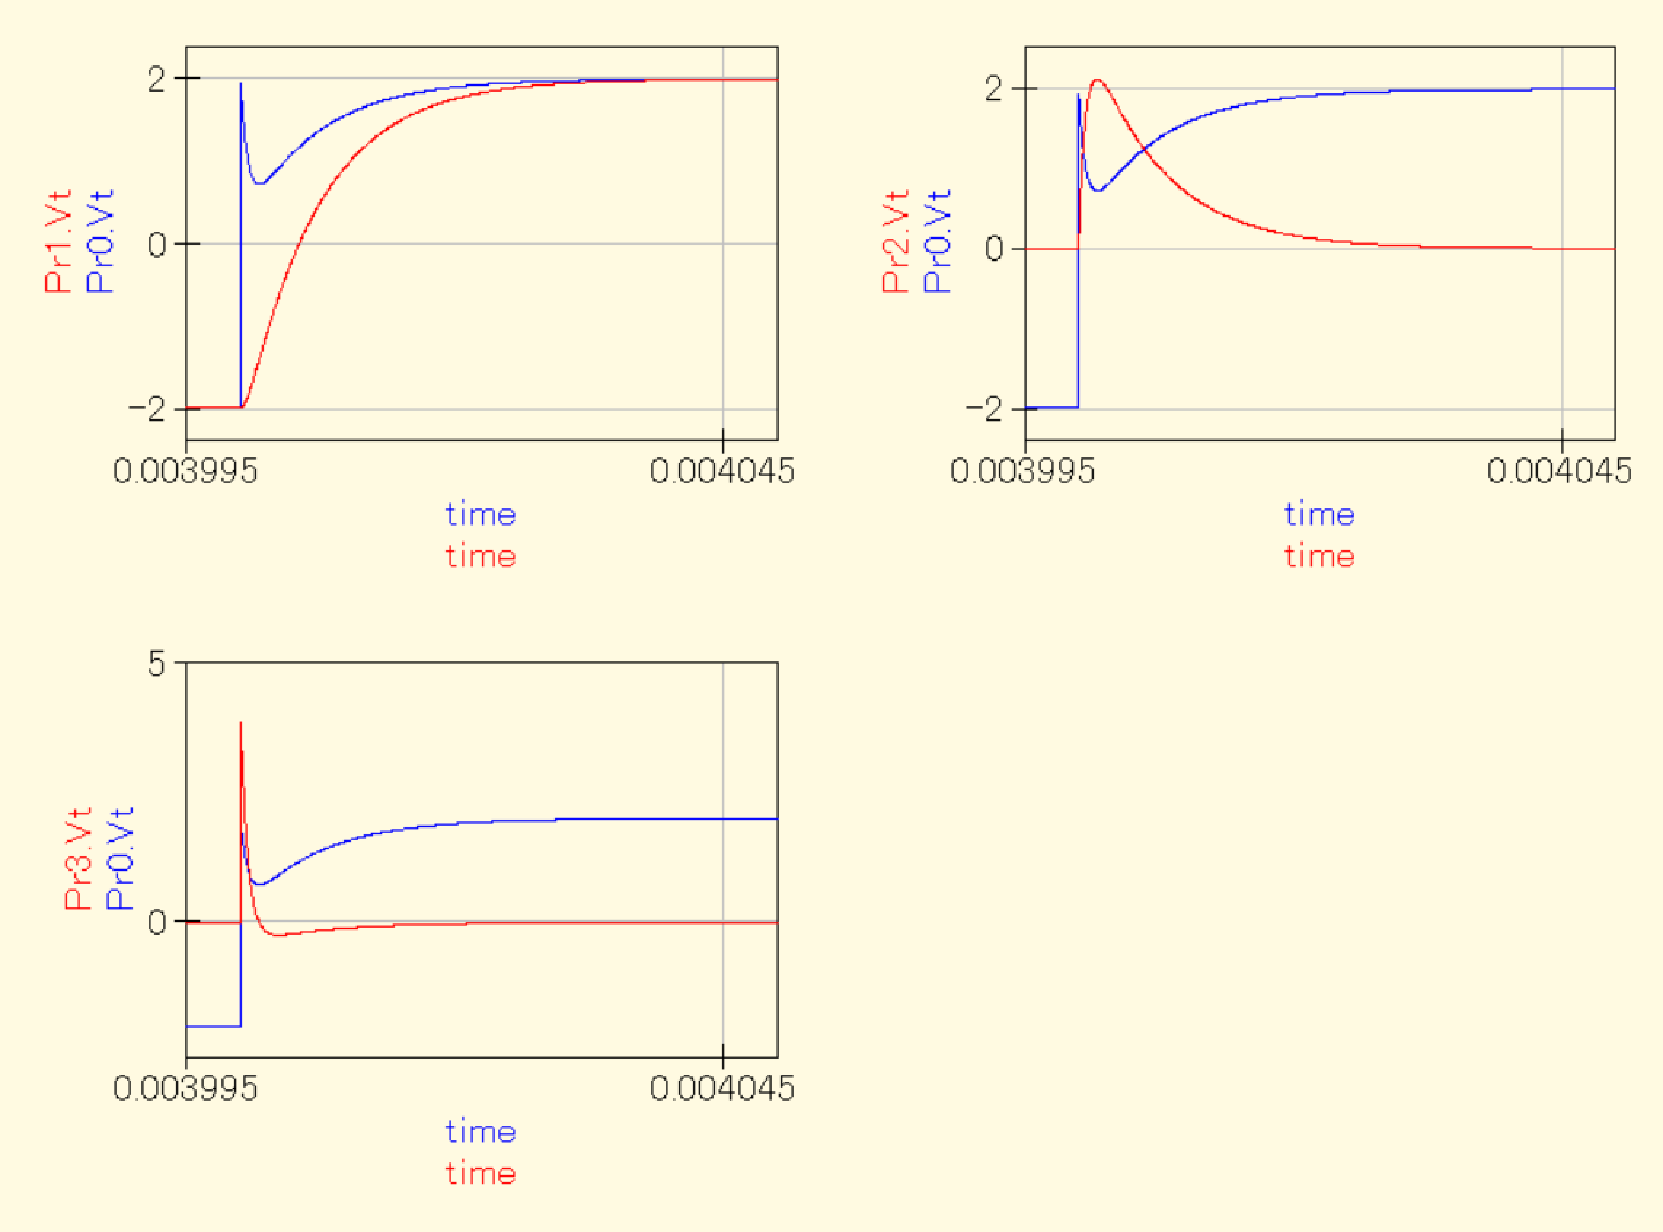
\includegraphics[keepaspectratio, scale=0.475]{result1.pdf}
        \caption{測定回路1のシミュレーション結果}
    \end{center}
\end{figure}

\begin{figure}[H]
    \begin{center}
        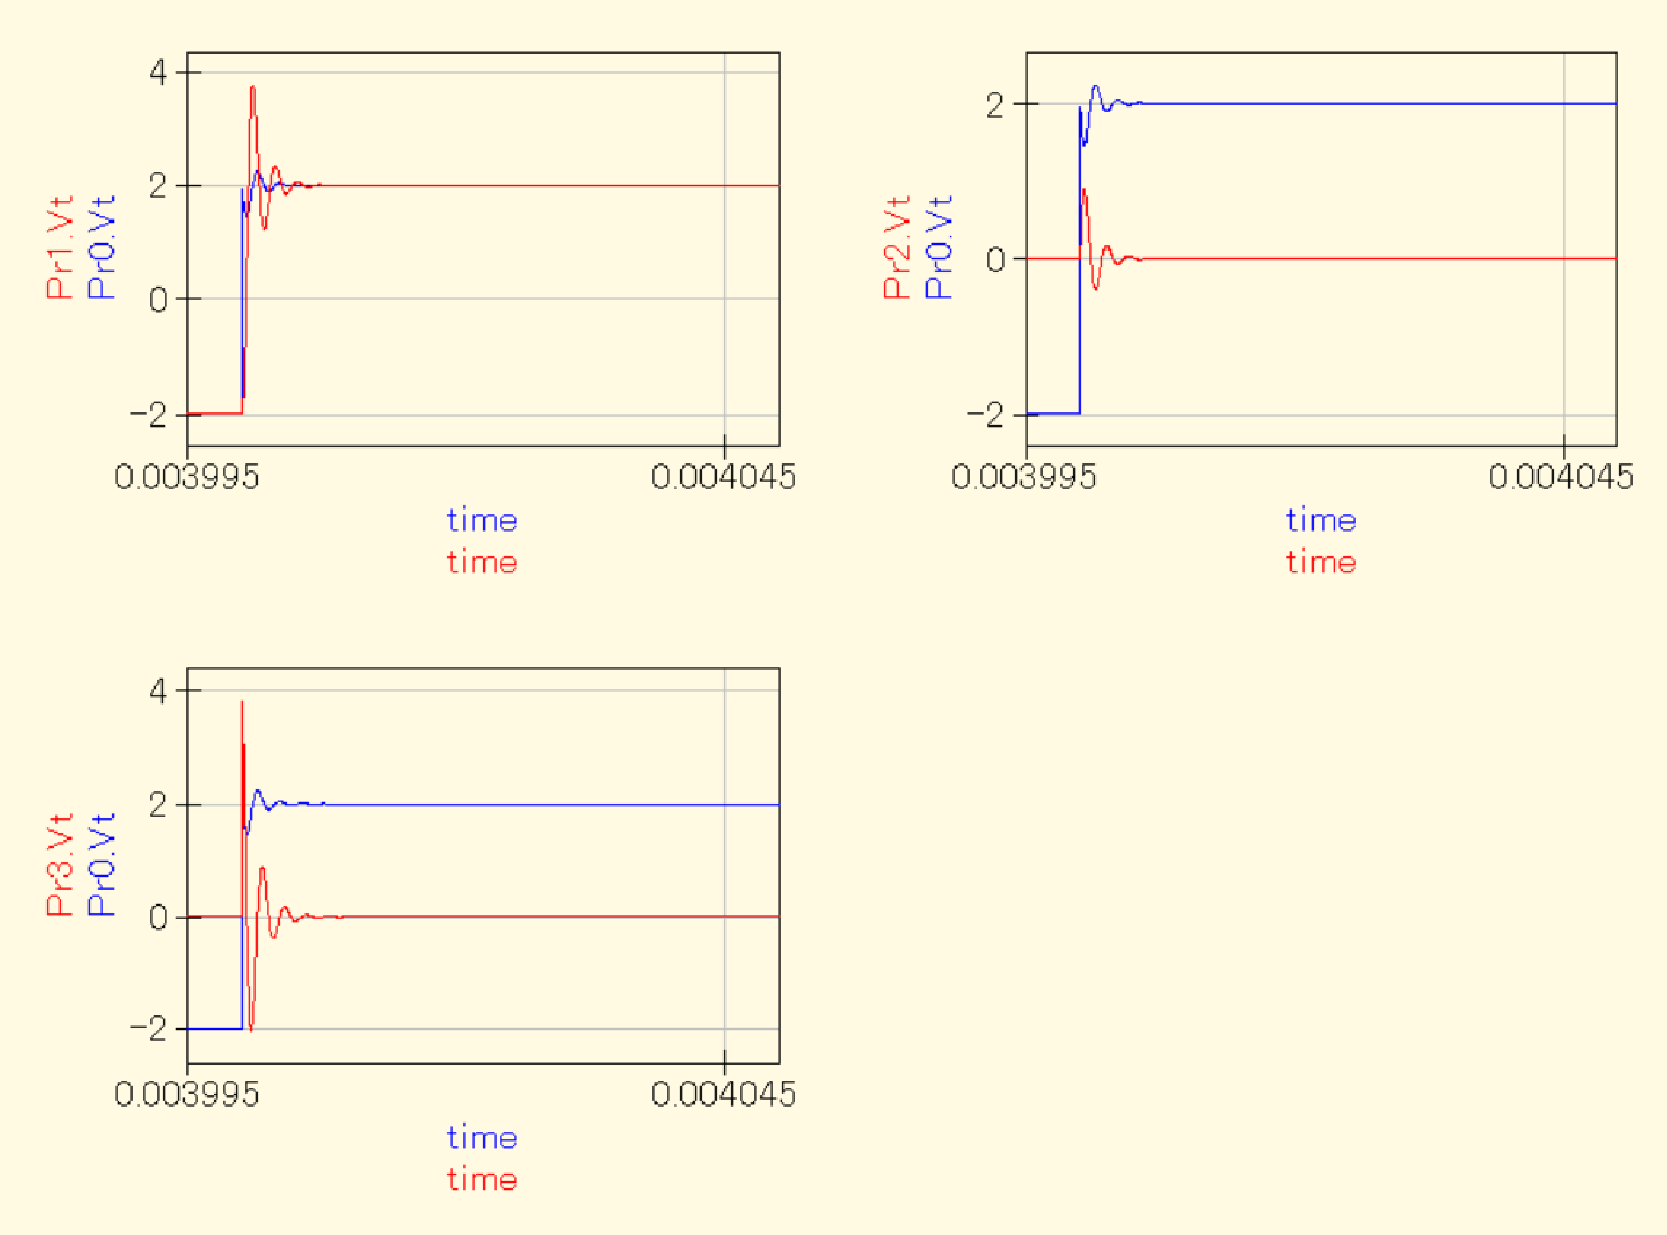
\includegraphics[keepaspectratio, scale=0.475]{result2.pdf}
        \caption{測定回路2のシミュレーション結果}
    \end{center}
\end{figure}

\subsection{測定波形}
\subsubsection{測定回路1}
測定回路1の測定測定波形を図9,図10,図11に示す.

\subsubsection{測定回路2}
測定回路1の測定測定波形を図12,図13,図14に示す.
